\documentclass[openright]{nkuthesis}
%%%%选项列表%%%%
% continum------------用于图表及公式的连续编号(章节无关)
% openright,openany---缺省为openany,用openright可保证每章在奇数页开始,打印时可选
% oneside,twoside-----缺省为twoside,双面格式,注意此项与openright相抵消
% appnum--------------附录参与计数
\usepackage[]{nkuthesistitle} %用LaTeX生成封面
%%%%选项列表%%%%
% dualdegree----------双学位选项,生成双学位用封面
\begin{document}

% 用户信息
% 作者姓名
\thesisauthor{XXX}
% 导师姓名
\teacher{XXX}
% 学号
\studentID{1111111}
% 年级
\grade{XXXX级}
%学院
\school{XXX学院}
%系别
\department{XXX系}
% 专业
\major{XXXX专业}
% 论文中英文标题
\thesistitle
{南开大学毕业论文模板模板模板模板模板模板模板模板模板模板模板模板}
{NKU thesis \LaTeX{} template test test test test test test test test test test test test}
% 毕设结束时间
\thesisend{2012}{07}{01}
% 论文签名时间
\thesisdate{2016}{04}{24}
%%%%%%%%%%%%%双修信息%%%%%%%%%%%%%
%双修院系
\dualschool{XXX}
%双修专业
\dualmajor{XXX}


%%%%%%%%%%%%%%%%%%%%%%%%%%%
% 封面
\frontmatter
\maketitle

% 声明页
\pagestyle{empty}
\cleardoublepage
\announce

% 摘要
\cleardoublepage
\setcounter{page}{1}
\pagestyle{plain}
% 中文摘要关键字
\chnkeyword{南开大学; 论文; 模版}
% 英文摘要关键字
\engkeyword{Nankai; Thesis}

% 中英文摘要
\begin{chnabstract}
这是NKUThesis模版的测试用文档,简单介绍了本模版的使用方法以及一些注意事项,本文档尚未完成。

测试用文字,测试用文字,测试用文字,测试用文字,测试用文字,测试用文字,测试用文字,测试用文字,测试用文字,测试用文字,测试用文字,测试用文字,测试用文字,测试用文字,测试用文字,测试用文字,测试用文字,测试用文字,测试用文字,测试用文字,测试用文字,测试用文字,测试用文字,测试用文字,测试用文字,测试用文字,测试用文字,测试用文字,测试用文字,测试用文字,测试用文字,测试用文字,测试用文字,测试用文字,测试用文字,测试用文字,测试用文字,测试用文字,测试用文字,测试用文字,测试用文字,测试用文字,测试用文字,测试用文字,测试用文字,测试用文字,测试用文字,测试用文字,测试用文字,测试用文字,测试用文字,测试用文字,测试用文字,测试用文字,测试用文字,测试用文字,测试用文字,测试用文字,测试用文字,测试用文字,测试用文字,测试用文字,测试用文字,测试用文字,测试用文字,测试用文字,测试用文字,测试用文字,测试用文字,测试用文字,测试用文字,测试用文字,测试用文字,测试用文字,测试用文字,测试用文字,测试用文字,测试用文字,测试用文字,测试用文字,测试用文字,测试用文字,测试用文字,测试用文字,测试用文字,测试用文字,测试用文字,测试用文字,测试用文字,测试用文字,测试用文字,测试用文字,测试用文字,测试用文字,测试用文字,测试用文字,测试用文字,测试用文字,测试用文字,测试用文字,测试用文字,测试用文字,测试用文字。
\end{chnabstract}

\begin{engabstract}
Here is the Abstract in English for test. The article explains the role and future trend of IT industry , and states that information technology represented by the internet and computers has brought about the third industrial revolution in history . An important impetus for economic growth in modern times , the IT industry has greatly promoted sustainable development and is profoundly changing mankind's way of life and production.

Test, test, test, test, test, test, test, test, test, test, test, test, test, test, test, test, test, test, test, test, test, test, test, test, test, test, test, test, test, test, test, test, test, test, test, test, test, test, test, test, test, test, test, test, test, test, test, test, test, test, test, test, test, test, test, test, test, test, test, test, test, test, test, test, test, test, test, test, test, test, test, test, test, test, test, test, test, test, test, test, test, test, test, test, test, test.
\end{engabstract}


%%%%%%%%%%%%%%%%%%%%%%%%%%%
% 目录
\tableofcontents

% 正文样式
\mainbody

% 正文
\chapter{简介}

\section{项目说明}

本项目为个人开发并维护的南开大学本科生毕业论文(设计)\LaTeX{}模版。

{\heiti 注意:本项目目前属于个人开发,时间、经历有限,目前仅可实现最基本功能,许多解决方案简单粗暴,可能存在各种潜在问题。使
用过程中有任何问题请及时与开发者联系。

欢迎有兴趣的同学加入本模版维护、扩展!}





\chapter{使用指南}

\section{脚注}
使用\textbackslash footnote来插入一个脚注\footnote{我是一条测试用的脚注}\footnote{真巧,我也是}\footnote{还有我}

\section{层级}
由于排版需要(懒得折腾)本模板只支持到subsection级别,标号规则遵从格式要求,如需要使用更深层标题,请改用列表环境并注意
指定所需格式。

\section{列表环境}

enumerate环境可以生成有序列表,默认序号格式如下:

\begin{enumerate}
\item 默认
\item 输出
\item 的
\item 列表
\end{enumerate}

通过控制label选项,可以输出不同格式的序号:

\begin{lstlisting}{language=TeX}
  \begin{enumerate}[label=(\arabic*)] % (1) (2) ...
\end{lstlisting}


下面是由此生成的列表

\begin{enumerate}[label=(\arabic*)]
\item 不同样子
\item 的
\item 列表
\end{enumerate}

无序号列表由itemize环境生成

\begin{itemize}
\item firstItem
\item seconItem
\item and so on
\end{itemize}

\section{代码环境示例}

下面是用listings包生成的一段C语言代码
\begin{lstlisting}{language=C}
if (i<=0) then i := 1;
if (i>=0) then i := 0;
if (i<>0) then i := 0;
\end{lstlisting}

\section{表格环境}

按规范,表格应为三线式,请依照格式制作表格\footnote{注释每页独立编号}

\begin{table}[htbp]
  \centering
  \caption{标题}
    \begin{tabular}{rrrrrr}
    \toprule
    test  & test  & test  & test  & test  & test \\
    \midrule
    test  & test  & test  & test  & test  & test \\
    test  & test  & test  & test  & test  & test \\
    test  & test  & test  & test  & test  & test \\
    test  & test  & test  & test  & test  & test \\
    test  & test  & test  & test  & test  & test \\
    test  & test  & test  & test  & test  & test \\
    \bottomrule
    \end{tabular}%
  \label{tab:addlabel}%
\end{table}%

\section{输入数学公式}
\begin{equation}
E=mc^2
\end{equation}

引用公式需要在标号外加括号,为了保证引用格式的正确,请使用amsmath包提供的 \textbackslash eqref来生成公式
引用而非\textbackslash ref

需要对齐的公式环境 \eqref{eq_test1} 到 \eqref{eq_test3}
\begin{align}
a &= 1 \label{eq_test1}\\
b &= 2 \label{eq_test2}\\
c &= 299792458\,\text{m/s} \label{eq_test3}
\end{align}

\section{带圈数字}
\textbackslash circnum通过映射数字实现了比较漂亮的带圈数字输出,主要用于注释及enumerate环境。
对于大于10的数字支持可能存在问题,请谨慎使用。

\begin{itemize}
  \item 1-10的数字将将其映射为对应字符\circnum{1}\circnum{2}\circnum{3}\circnum{4}\circnum{5}\circnum{6}\circnum{7}\circnum{8}\circnum{9}\circnum{10}
  \item 其余数字利用\textbackslash textcircled加框,同时对数字位置作了微调\circnum{0}\circnum{20}\circnum{99}
\end{itemize}

\section{插图示例}

\begin{figure}[htbp]
  \centering
  \subfigure[高德纳]{ 
    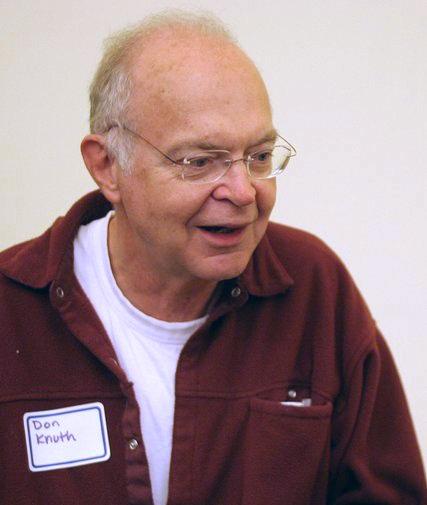
\includegraphics[height=6cm]{figure/Knuth.jpg}
  }
  \subfigure[莱斯利·兰波特]{ 
    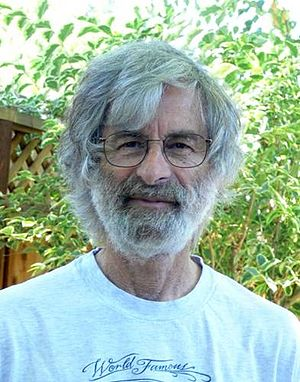
\includegraphics[height=6cm]{figure/Leslie_Lamport.jpg}
  }
  \caption{高德纳和莱斯利·兰波特,\TeX{}和\LaTeX{}的开发者}
\end{figure}

\section{参考文献}
参考文献格式部分参考了\href{https://github.com/ustctug/gbt-7714-2015}{GB/T 7714-2015 BibTeX Style},并进行了一部分改动,
整理比较仓促,如使用中发现了问题,请尽快与作者联系。

\section{长表格}

跨页长表格用longtable环境产生,请参考表 \ref{tab-data}进行长表格制作。

\begin{center}
\begin{longtable}{lrr}
\caption{我是一个长表格}\label{tab-data}\\
\toprule
Sample  & Sample & Sample \\
\midrule
\endfirsthead
\multicolumn{3}{c}{\hfill (接上页) \hfill 续表 \ref{tab-data}}\\
\toprule
Sample  & Sample & Sample \\
\midrule
\endhead
\bottomrule
\multicolumn{3}{c}{(接下页)}
\endfoot
\bottomrule
\endlastfoot
1234567 & 2     & 3.00000000000000E+00 \\
1234567 & 4     & 9.00000000000000E+00 \\
1234567 & 8     & 2.70000000000000E+01 \\
1234567 & 16    & 8.10000000000000E+01 \\
1234567 & 32    & 2.43000000000000E+02 \\
1234567 & 64    & 7.29000000000000E+02 \\
1234567 & 128   & 2.18700000000000E+03 \\
1234567 & 256   & 6.56100000000000E+03 \\
1234567 & 512   & 1.96830000000001E+04 \\
1234567 & 1024  & 5.90490000000003E+04 \\
1234567 & 2048  & 1.77147000000001E+05 \\
1234567 & 4096  & 5.31441000000003E+05 \\
1234567 & 8192  & 1.59432300000001E+06 \\
1234567 & 16384 & 4.78296900000003E+06 \\
1234567 & 32768 & 1.43489070000001E+07 \\
1234567 & 65536 & 4.30467210000003E+07 \\
1234567 & 131072 & 1.29140163000001E+08 \\
1234567 & 262144 & 3.87420489000003E+08 \\
1234567 & 524288 & 1.16226146700001E+09 \\
1234567 & 1048576 & 3.48678440100003E+09 \\
1234567 & 2097152 & 1.04603532030001E+10 \\
1234567 & 4194304 & 3.13810596090003E+10 \\
1234567 & 8388608 & 9.41431788270006E+10 \\
1234567 & 16777216 & 2.82429536481002E+11 \\
1234567 & 33554432 & 8.47288609443006E+11 \\
1234567 & 67108864 & 2.54186582832902E+12 \\
1234567 & 134217728 & 7.62559748498706E+12 \\
1234567 & 268435456 & 2.28767924549612E+13 \\
1234567 & 72434964.49 & 6.86303773648836E+13 \\
1234567 & 76108137.14 & 2.05891132094651E+14 \\
1234567 & 79781309.79 & 6.17673396283953E+14 \\
1234567 & 83454482.44 & 1.85302018885186E+15 \\
1234567 & 87127655.09 & 5.55906056655558E+15 \\
1234567 & 90800827.74 & 1.66771816996667E+16 \\
1234567 & 94474000.39 & 5.00315450990001E+16 \\
1234567 & 98147173.04 & 1.50094635297001E+17 \\
1234567 & 101820345.7 & 4.50283905891003E+17 \\
1234567 & 105493518.3 & 1.35085171767301E+18 \\
1234567 & 109166691 & 4.05255515301903E+18 \\
1234567 & 112839863.6 & 1.21576654590571E+19 \\
1234567 & 116513036.3 & 3.64729963771713E+19 \\
1234567 & 120186208.9 & 1.09418989131514E+20 \\
1234567 & 123859381.6 & 3.28256967394542E+20 \\
1234567 & 127532554.2 & 9.84770902183626E+20 \\
1234567 & 131205726.9 & 2.95431270655087E+21 \\
1234567 & 134878899.5 & 8.86293811965264E+21 \\
1234567 & 138552072.2 & 2.65888143589579E+22 \\
1234567 & 142225244.8 & 7.97664430768737E+22 \\
1234567 & 145898417.5 & 2.39299329230621E+23 \\
1234567 & 149571590.1 & 7.17897987691863E+23 \\
1234567 & 153244762.8 & 2.15369396307559E+24 \\
1234567 & 156917935.4 & 6.46108188922677E+24 \\
1234567 & 160591108.1 & 1.93832456676803E+25 \\
1234567 & 164264280.7 & 5.81497370030409E+25 \\
1234567 & 167937453.4 & 1.74449211009123E+26 \\
1234567 & 171610626 & 5.23347633027369E+26 \\
1234567 & 175283798.7 & 1.57004289908211E+27 \\
\end{longtable}
\end{center}


\chapter{English Example}

本章展示了模版对英文的支持情况,英文字体为 Times New Roman,为了调用系统字体,必须使用XeLaTeX或者LuaLaTeX编译。

\section{Gettysburg Address}

Four score and seven years ago our fathers brought forth, upon this continent, a new nation, conceived in liberty, and dedicated to the proposition that "all men are created equal"

Now we are engaged in a great civil war, testing whether that nation, or any nation so conceived, and so dedicated, can long endure. We are met on a great battle field of that war. We have come to dedicate a portion of it, as a final resting place for those who died here, that the nation might live. This we may, in all propriety do. But, in a larger sense, we can not dedicate—we can not consecrate—we can not hallow, this ground—The brave men, living and dead, who struggled here, have hallowed it, far above our poor power to add or detract. The world will little note, nor long remember what we say here; while it can never forget what they did here.

It is rather for us, the living, to stand here, we here be dedicated to the great task remaining before us—that, from these honored dead we take increased devotion to that cause for which they here, gave the last full measure of devotion—that we here highly resolve these dead shall not have died in vain; that the nation, shall have a new birth of freedom, and that government of the people by the people for the people, shall not perish from the earth.


%%%%%%%%%%%%%%%%%%%%%%%%%%%
% 附录
\appendix
\chapter{附~~~~录}
\label{chapter-faq}

\section{常见问题}
\begin{enumerate}
\item 使用中报错或发现问题怎么办?
    
    请发邮件至\url{jeffrey.wei.jh@gmail.com}, 我会尽(jin)快(liang)回复。 
    一个人精力有限,希望更多的人能够加入到模版的开发中来。
\item 我用CTeX套装编译不通过怎么办
     
     CTeX 套装已经年久失修,不建议大家继续使用(最近倒是说要出新版),可以根据自身系统
     安装\TeX{} Live 或Mac\TeX{} ,这些成熟的发行版都自带包管理器,与中文格式相关的
     CTeX 包也在仓库中予以提供,唯一的缺点就是完全安装的话体积太大。XeLaTeX 是现在处
     理CJK 字符的较成熟方案,所以请使用XeLaTeX 编译。
    
\end{enumerate}
    

\section{其他}
来,大家和我一起吐槽
\begin{itemize}
\item 带圈的数字很太丑了,标号规则不能改改么!!!
\item 论文指导手册提供的封面尺寸不是A4纸!!!白瞎我照着改了半天......
\item 1.5倍行距这东西放到\LaTeX{}下面是个大坑!!!
\item 为什么默认格式是啥格式手册就要弄个不一样要求的出来!!!
\item 封面太难做了!!!是我用尺量着做出来的......
\item 论文还没写完!!!!!!!
\end{itemize}

折腾排版这东西确实容易让人有种想杀人的冲动......


% 参考文献
\cleardoublepage
\phantomsection
\addcontentsline{toc}{chapter}{参考文献}
\nocite{*}
\bibliography{main/bibliography}
\cleardoublepage


% 致谢
\chapter*{致~~~~谢}
\addcontentsline{toc}{chapter}{致谢}
一点微小的工作,谢谢大家
\cleardoublepage


\end{document}
